\documentclass[aps,prd,twocolumn,superscriptaddress,nofootinbib,floatfix]{revtex4-2}

\usepackage{fontspec}
\defaultfontfeatures{Ligatures=TeX}
\usepackage{polyglossia}
\setdefaultlanguage{russian}
\setotherlanguage{english}
\setmainfont{Times New Roman}
\setsansfont{Arial}
\setmonofont{Courier New}
\newfontfamily\cyrillicfont{Times New Roman}
\newfontfamily\cyrillicfontsf{Arial}
\newfontfamily\cyrillicfonttt{Courier New}
\usepackage{amsmath,amssymb}
\usepackage{mathtools}
\usepackage{booktabs}
\usepackage{graphicx}
\usepackage{hyperref}
\usepackage{xcolor}
\usepackage{slashed}
\usepackage{amsthm}
\newtheorem{theorem}{\cyrillicfont Теорема}[section]
\newtheorem{proposition}[theorem]{\cyrillicfont Предложение}
\newtheorem{lemma}[theorem]{\cyrillicfont Лемма}
\newtheorem{corollary}[theorem]{\cyrillicfont Следствие}
\theoremstyle{definition}
\newtheorem{definition}[theorem]{\cyrillicfont Определение}
\theoremstyle{remark}
\newtheorem{remark}[theorem]{\cyrillicfont Замечание}

\hypersetup{
  colorlinks=true,
  linkcolor=blue!60!black,
  citecolor=blue!60!black,
  urlcolor=blue!60!black,
  pdfauthor={Давид Алфёров},
  pdftitle={Нелокальные однопетлевые формфакторы спектрального действия с содержанием частиц Стандартной модели},
  pdfsubject={doi:10.22541/au.177507193.33027854/v1}
}

%%% Custom commands
\newcommand{\Weylsq}{C_{\mu\nu\rho\sigma}C^{\mu\nu\rho\sigma}}
\newcommand{\Ricsq}{R_{\mu\nu}R^{\mu\nu}}
\newcommand{\Riemsq}{R_{\mu\nu\rho\sigma}R^{\mu\nu\rho\sigma}}
\newcommand{\dd}{\mathrm{d}}
\newcommand{\erfi}{\operatorname{erfi}}
\newcommand{\tr}{\operatorname{tr}}
\newcommand{\Tr}{\operatorname{Tr}}

\begin{document}

\title{Нелокальные однопетлевые формфакторы спектрального действия\\с содержанием частиц Стандартной модели}

\author{Давид Алфёров}
\affiliation{Независимый исследователь}
\email{davidich.alfyorov@gmail.com}

\begin{abstract}
Мы вычисляем индуцированные материей нелокальные однопетлевые квадратичные
по кривизне формфакторы $F_1(\Box/\Lambda^2)$ и $F_2(\Box/\Lambda^2,\xi)$,
относящиеся к спектральному действию
$S = \Tr\,f(D^2/\Lambda^2)$, для содержания полей Стандартной модели:
4 вещественных скаляра (дублет Хиггса), $45/2$ дираковских фермионов
(3 поколения) и 12 калибровочных бозонов
($\mathrm{SU}(3)\times\mathrm{SU}(2)\times\mathrm{U}(1)$).
С~помощью ковариантной теории возмущений
Барвинского--Вилковыского~\cite{Barvinsky:1985an,Barvinsky:1987uw}
и нелокального ядра теплопроводности
Коделло--Занусси~\cite{Codello:2012kq} мы выводим замкнутые выражения
для приведённых ядер $h_C^{(s)}(x)$ и $h_R^{(s)}(x)$ для каждого спинового
сектора ($s = 0, 1/2, 1$) в вейлевском базисе $\{C^2, R^2\}$
с~пошаговой сборкой из пяти универсальных структурных функций КЗ. Для
спина~1 приведён полный вывод духов Фаддеева--Попова с~двумя минимально
связанными скалярными духами. Сборка Стандартной модели даёт
$\alpha_C = 13/120$ (квадрат тензора Вейля, не зависит от~$\xi$) и
$\alpha_R(\xi) = 2(\xi - 1/6)^2$ ($R^2$, зависит только от неминимальной
связи Хиггса), воспроизводя все известные локальные
пределы~\cite{Gilkey:1975iq,Vassilevich:2003xt,Codello:2008vh,Stelle:1976gc}.
После устранения кажущихся особенностей при $z = 0$ доказано, что приведённые
формфакторы являются целыми функциями переменной $z = \Box/\Lambda^2$ порядка~1
и типа~$1/4$; следовательно, сами формфакторы не вносят полюсов в пропагатор.
Полюса духов возникают из нулей одетого пропагатора, который мы выводим
из полного линеаризованного квадратичного действия с~помощью спиновых
проекторов Барнса--Риверса~\cite{Barnes:1965,Rivers:1964}. Это даёт эффективные
массы $m_2 = \Lambda\sqrt{60/13}$ (спин~2) и
$m_0 = \Lambda/\sqrt{6(\xi - 1/6)^2}$ (спин~0), причём скалярная мода
отщепляется при конформной связи $\xi = 1/6$.
Все результаты независимо верифицированы тройной компьютерной алгеброй
(SymPy, cadabra2~\cite{Peeters:2007wn}, FORM~\cite{Vermaseren:2000nd}),
численной оценкой с~произвольной точностью ($\geq 100$ цифр) и формальными
доказательствами на Lean~4 для арифметики коэффициентов.
\end{abstract}

\pacs{04.62.+v, 04.60.-m, 11.10.Jj, 04.50.Kd}
\keywords{спектральное действие, ядро теплопроводности, формфакторы,
квадратичная гравитация, Стандартная модель, некоммутативная геометрия}

\maketitle

% ============================================================
\section{Введение}
\label{sec:intro}
% ============================================================

Принцип спектрального действия~\cite{Connes:1994yd,Chamseddine:1996zu,Chamseddine:2006ep}
обеспечивает геометрическое происхождение как гравитационных, так и
калибровочных взаимодействий: бозонное действие задаётся выражением
$S = \Tr\,f(D^2/\Lambda^2)$, где $D$ --- оператор Дирака некоммутативной
геометрии, $\Lambda$ --- масштаб обрезания, а $f$ --- положительная чётная
функция. На классическом уровне разложение этого следа по ядру
теплопроводности воспроизводит действие Эйнштейна--Гильберта, космологическую
постоянную и члены Янга--Миллса из первых нескольких коэффициентов
Сили--Де Витта~\cite{Chamseddine:2010ud,vanSuijlekom:2014pya}.

За рамками ведущего приближения Сили--Де Витта спектральное действие порождает
\emph{нелокальные} квадратичные по кривизне члены, характеризуемые зависящими
от импульса формфакторами $F_1(\Box/\Lambda^2)$ и $F_2(\Box/\Lambda^2,\xi)$.
Эти формфакторы кодируют \emph{индуцированный материей} вклад в однопетлевое
квадратичное по кривизне эффективное действие порядка
$\mathcal{O}(\mathcal{R}^2)$: они возникают из функциональных следов по полям
материи (скаляры, фермионы, калибровочные бозоны), распространяющимся на
фиксированном искривлённом гравитационном фоне. Вклады собственной энергии
гравитона, которые составили бы полное квантово-гравитационное эффективное
действие, здесь не вычисляются; они требуют отдельного рассмотрения оператора
метрических флуктуаций, его фиксации калибровки и гравитационного сектора
духов~\cite{Stelle:1976gc,Buchbinder:1992rb}. Тем не менее индуцированные
материей формфакторы уже определяют структуру модифицированного пропагатора
гравитона, эффективные массы и ультрафиолетовое поведение в режиме
доминирования материальных петель.

Ковариантная теория возмущений Барвинского--Вилковыского
(БВ)~\cite{Barvinsky:1985an,Barvinsky:1987uw,Barvinsky:1990up,Barvinsky:2009gw}
предоставляет общий формализм для вычисления таких формфакторов для
произвольного обобщённого лапласиана
$\Delta = -(g^{\mu\nu}\nabla_\mu\nabla_\nu + E)$ на векторном расслоении
над искривлённым многообразием. Диаграммная техника ядра теплопроводности
Коделло--Занусси (КЗ)~\cite{Codello:2012kq} даёт явные выражения для пяти
независимых структурных функций
($f_{\text{Ric}}, f_R, f_{RU}, f_U, f_\Omega$) через универсальную
мастер-функцию $\varphi(x)$, которая зависит только от параметра собственного
времени и не зависит от профильной функции $f$ при
$\mathcal{O}(\mathcal{R}^2)$ (доказательство см. в приложении~\ref{app:profile}).
Коэффициенты Сили--Де Витта и их роль в спектральной геометрии
рассмотрены
в~\cite{DeWitt:1964mxt,Gilkey:1975iq,Vassilevich:2003xt,Avramidi:2000bm,Fursaev:2011zz}.

Формфакторы для отдельных лапласианов были получены
БВ~\cite{Barvinsky:1987uw,Barvinsky:1990up} и
КЗ~\cite{Codello:2012kq}; локальные пределы (коэффициенты $\beta$-функций)
были табулированы для полей материи КПР~\cite{Codello:2008vh} и в учебнике
Паркера и Томса~\cite{Parker:2009uva}. Однопетлевые поправки к спектральному
действию были изучены ван Нуландом и ван
Сёйлекомом~\cite{vanNuland:2022xkm}, а рамки спектрального действия для
высшепроизводной гравитации были проанализированы Мистри, Пинзулом и
Рахвалом~\cite{Mistry:2020xqh}. Настоящая работа собирает полные формфакторы
Стандартной модели (СМ) для каждого спинового сектора в специфичные для СМ
величины ($\alpha_C$, $\alpha_R(\xi)$, $c_1/c_2$), которые ранее не
приводились, доказывает свойство целой функции для полных сумм СМ и выводит
одетый пропагатор гравитона из полного линеаризованного квадратичного действия.

Содержание частиц СМ состоит из 4~вещественных скаляров (дублет Хиггса),
$N_f = 45$ вейлевских фермионов (что эквивалентно $N_D = 45/2$ дираковским
фермионам в 3~поколениях) и 12~калибровочных бозонов группы
$\mathrm{SU}(3) \times \mathrm{SU}(2) \times \mathrm{U}(1)$. Соглашение
о~подсчёте следует КПР~\cite{Codello:2008vh}.

Основные результаты:
\begin{itemize}
\item Замкнутые выражения для приведённых формфакторов
  $h_C^{(s)}(x)$ и $h_R^{(s)}(x)$ при $s = 0, 1/2, 1$ в вейлевском базисе
  $\{C^2, R^2\}$ с~полным пошаговым выводом сборки БВ/КЗ для каждого
  спинового сектора (разд.~\ref{sec:scalar}--\ref{sec:vector}).
\item Полные суммы СМ: $\alpha_C = 13/120$ (не зависит от~$\xi$,
  определяется содержанием СМ) и $\alpha_R(\xi) = 2(\xi - 1/6)^2$
  (зависит только от неминимальной связи Хиггса~$\xi$), причём
  локальный коэффициент при $R^2$ обращается в нуль при конформной
  связи $\xi = 1/6$ (разд.~\ref{sec:sm}).
\item Доказательство того, что приведённые формфакторы после
  устранения кажущихся особенностей при $z = 0$ являются целыми
  функциями порядка~1 и типа~$1/4$ (теорема~\ref{thm:entire}).
  Как следствие, формфакторы не вносят полюсов в пропагатор; полюса
  духов возникают исключительно из нулей одетого пропагатора
  (разд.~\ref{sec:entire}).
\item Одетые пропагаторы спина~2 и спина~0:
  $\Pi_{TT}(z)$, $\Pi_s(z,\xi)$, выведенные из полного линеаризованного
  квадратичного действия с~помощью проекторов Барнса--Риверса, с
  эффективными массами $m_2 = \Lambda\sqrt{60/13}$,
  $m_0 = \Lambda/\sqrt{6(\xi - 1/6)^2}$ и модифицированным ньютоновским
  потенциалом (разд.~\ref{sec:propagator}).
\item Систематическое сравнение с~БВ, КЗ, КПР, Паркером--Томсом,
  Стелле и эффективной теорией поля
  Донохью~\cite{Donoghue:1994dn,BjerrumBohr:2002kt}
  (разд.~\ref{sec:comparison}).
\end{itemize}

Структура статьи следующая. В~разделе~\ref{sec:setup} устанавливаются
соглашения и излагается формализм БВ/КЗ, включая $f$-независимость
формфакторов при $\mathcal{O}(\mathcal{R}^2)$.
В~разделах~\ref{sec:scalar}--\ref{sec:vector} выводятся формфакторы для
каждого спинового сектора с~явной сборкой БВ.
В~разделе~\ref{sec:sm} собираются полные суммы СМ.
В~разделе~\ref{sec:entire} доказывается свойство целой функции.
В~разделе~\ref{sec:propagator} выводятся одетый пропагатор и эффективные
массы. В~разделе~\ref{sec:uv} обсуждается ультрафиолетовая асимптотика.
В~разделе~\ref{sec:comparison} проводится сравнение с~существующими
результатами, включая ЭТП Донохью. В~разделе~\ref{sec:discussion}
обсуждаются следствия для асимптотической безопасности и нелокальной
гравитации. Заключение приведено в~разд.~\ref{sec:conclusions}.

В~данной статье мы используем евклидову сигнатуру $(+,+,+,+)$, естественные
единицы $c = \hbar = 1$ и соглашение для обобщённого лапласиана
$\Delta = -(g^{\mu\nu}\nabla_\mu\nabla_\nu + E)$ Барвинского и
Вилковыского~\cite{Barvinsky:1985an}. Эндоморфизм КЗ есть
$\mathbf{U} = -E$. Лоренцево продолжение к сигнатуре $(-,+,+,+)$
обсуждается в~разд.~\ref{sec:discussion}. Таблицы соглашений собраны
в~приложении~\ref{app:conventions}. Сводка основных результатов приведена
в~таблице~\ref{tab:summary}.


% ============================================================
\section{Постановка задачи и соглашения}
\label{sec:setup}
% ============================================================

\subsection{Обобщённый лапласиан и спектральное действие}

Рассмотрим замкнутое (компактное, без края) римановое спиновое
4-многообразие $(M,g)$. Для каждого поля материи спина~$s$ однопетлевое
эффективное действие имеет вид
\begin{equation}
  \Gamma^{(s)} = \frac{(-1)^{2s}}{2}\,\Tr\ln\Delta^{(s)}\,,
  \label{eq:one-loop}
\end{equation}
где $\Delta^{(s)}$ --- обобщённый лапласиан соответствующего кинетического
оператора, а $(-1)^{2s} = +1$ для бозонов, $-1$ для фермионов. В~порядке
$\mathcal{O}(\mathcal{R}^2)$ квадратичный по кривизне сектор эффективного
действия принимает вид
\begin{equation}
  \Gamma\Big|_{\mathcal{R}^2}
  = \int_M \dd^4x\,\sqrt{g}\,\bigl[
    F_1(z)\,\Weylsq + F_2(z,\xi)\,R^2
  \bigr]\,,
  \label{eq:spectral-action}
\end{equation}
где $z \equiv \Box/\Lambda^2$ и $\Lambda$ --- спектральный масштаб обрезания.
Формфакторы $F_i$ являются центральными объектами данной работы.

Для обобщённого лапласиана $\Delta = -(g^{\mu\nu}\nabla_\mu\nabla_\nu + E)$,
действующего на векторном расслоении ранга $d_V$ (так что
$\tr\,\mathbf{1} = d_V$), эндоморфизм КЗ равен $\mathbf{U} = -E$, а
кривизна расслоения --- $\Omega_{\mu\nu} = [\nabla_\mu, \nabla_\nu]$,
действующая на сечениях расслоения. Мы записываем
\begin{equation}
  F_i^{(s)}(z) = \frac{h_i^{(s)}(z)}{16\pi^2}\,,\quad i = C, R\,,
  \label{eq:Fi-hi-def}
\end{equation}
где $h_C^{(s)}$ и $h_R^{(s)}$ --- \emph{приведённые} формфакторы.
Их локальные пределы $\beta_W^{(s)} \equiv h_C^{(s)}(0)$ и
$\beta_R^{(s)} \equiv h_R^{(s)}(0)$ суть однопетлевые коэффициенты
$\beta$-функции операторов $C^2$ и $R^2$. В~нашем соглашении фермионный
знак из~\eqref{eq:one-loop} не применяется как дополнительный общий
множитель; он закодирован в правилах сборки через операторные данные
(разд.~\ref{sec:assembly}). Для спинов СМ $s = 0, 1/2, 1$ результирующий
$h_C^{(s)}(0)$ положителен для бозонов и отрицателен для дираковского
фермиона, однако эта закономерность не распространяется на все спины
(см. разд.~\ref{sec:rs}).

\subsection{От ядер теплопроводности к формфакторам спектрального действия}
\label{sec:smearing}

Спектральное действие $S = \Tr\,f(D^2/\Lambda^2)$ зависит от профильной
функции~$f$. Уточним теперь, как формфакторы зависят от~$f$ и при каких
условиях они $f$-независимы.

Если $f$ допускает представление Лапласа
$f(u) = \int_0^\infty \dd\alpha\,\tilde{f}(\alpha)\,e^{-\alpha u}$,
то спектральное действие при $\mathcal{O}(\mathcal{R}^2)$ принимает вид
\begin{align}
  S_f\big|_{\mathcal{R}^2}
  &= \frac{1}{16\pi^2}\int_M \dd^4x\,\sqrt{g}\,\bigl[
    \mathcal{H}_C(z;f)\,\Weylsq
  \nonumber\\
  &\qquad + \mathcal{H}_R(z,\xi;f)\,R^2
  \bigr]\,,
  \label{eq:smeared-action}
\end{align}
где \emph{усреднённые по профилю} формфакторы суть
\begin{equation}
  \mathcal{H}_i(z;f) = \int_0^\infty \dd\alpha\,\tilde{f}(\alpha)\,
    h_i(\alpha z)\,,\quad i = C,R\,.
  \label{eq:smearing}
\end{equation}
Здесь $h_i$ обозначает \emph{приведённое ядро}, соответствующее
экспоненциальному профилю $f(u) = e^{-u}$ (т.\,е.\
$\tilde{f}(\alpha) = \delta(\alpha - 1)$). Приведённые ядра, построенные
из мастер-функции $\varphi(x)$, универсальны --- они зависят только от
оператора типа Лапласа и не зависят от спектрального профиля. Зависимость
от профиля входит исключительно через размазывание~\eqref{eq:smearing}.

\begin{remark}
Все явные замкнутые формулы в данной статье представляют собой приведённые
ядра $h_i$. Они совпадают с формфакторами спектрального действия только
для экспоненциального профиля или, более общо, для любой меры собственного
времени с~дельта-функционным носителем.
\end{remark}

Непосредственным следствием~\eqref{eq:smearing} является зависимость
локальных коэффициентов от профиля:
\begin{equation}
  \mathcal{H}_i(0;f) = h_i(0)\,f(0)\,,
  \label{eq:f0-factor}
\end{equation}
поскольку $\int_0^\infty \tilde{f}(\alpha)\,\dd\alpha = f(0)$.
Следовательно, \emph{отношения} локальных квадратичных по кривизне
связей (например, $c_1/c_2$) не зависят от профиля, тогда как общая
нормировка пропорциональна $f(0)$. Для локальных коэффициентов СМ:
\begin{equation}
  \alpha_C^{\text{loc}} = \frac{13}{120}\,f(0)\,,\qquad
  \alpha_R^{\text{loc}} = 2\,f(0)\!\left(\xi - \frac{1}{6}\right)^{\!2}\,.
  \label{eq:alphaC-local-f}
\end{equation}
В~данной статье мы полагаем $f(0) = 1$ (экспоненциальный профиль), если не
оговорено иное.

\subsection{Мастер-функция}

Все формфакторы строятся из универсальной мастер-функции
\begin{equation}
  \varphi(x) = \int_0^1 \dd\alpha\, e^{-\alpha(1-\alpha)x}\,,
  \label{eq:phi-def}
\end{equation}
имеющей замкнутую форму
\begin{equation}
  \varphi(x) = e^{-x/4}\sqrt{\frac{\pi}{x}}\;\erfi\!\left(\frac{\sqrt{x}}{2}\right)\,.
  \label{eq:phi-closed}
\end{equation}
Основные свойства:
$\varphi(0) = 1$,
$\varphi'(0) = -1/6$,
тейлоровские коэффициенты $a_n = (-1)^n\,n!/(2n+1)!$, так что
$\varphi(x) = \sum_{n=0}^\infty a_n\,x^n$ с бесконечным радиусом
сходимости (признак Даламбера даёт $|a_{n+1}/a_n| \to 0$). В~частности,
$\varphi$ является целой функцией порядка~1 и типа~$1/4$
(рис.~\ref{fig:phi}). Асимптотическое разложение при больших~$x$:
\begin{equation}
  \varphi(x) = \frac{2}{x} + \frac{4}{x^2} + \frac{24}{x^3}
    + \frac{240}{x^4} + \mathcal{O}(x^{-5})\,,
  \label{eq:phi-uv}
\end{equation}
которое представляет собой асимптотический (расходящийся) ряд,
борелевски суммируемый к точной функции~$\varphi$.

\begin{figure}[t]
  \centering
  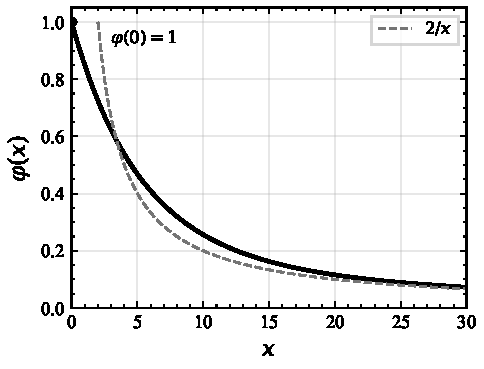
\includegraphics[width=\columnwidth]{figures/fig_phi_ru.pdf}
  \caption{Мастер-функция $\varphi(x)$, где
  $x = \Box/\Lambda^2$. Начиная с~$\varphi(0) = 1$, функция
  монотонно убывает и стремится к асимптотической форме $2/x$
  (штриховая линия) при $x \gg 1$.}
  \label{fig:phi}
\end{figure}

\subsection{Структурные функции КЗ}

Пять структурных функций КЗ~\cite{Codello:2012kq}:
\begin{subequations}
\label{eq:CZ-ff}
\begin{align}
  f_{\text{Ric}}(x) &= \frac{1}{6x} + \frac{\varphi - 1}{x^2}\,,
  \label{eq:fRic}\\
  f_R(x) &= \frac{\varphi}{32} + \frac{\varphi}{8x}
    - \frac{7}{48x} - \frac{\varphi - 1}{8x^2}\,,
  \label{eq:fR}\\
  f_{RU}(x) &= -\frac{\varphi}{4} - \frac{\varphi - 1}{2x}\,,
  \label{eq:fRU}\\
  f_U(x) &= \frac{\varphi}{2}\,,
  \label{eq:fU}\\
  f_\Omega(x) &= -\frac{\varphi - 1}{2x}\,.
  \label{eq:fOmega}
\end{align}
\end{subequations}
Их локальные пределы: $f_{\text{Ric}}(0) = 1/60$, $f_R(0) = 1/120$,
$f_{RU}(0) = -1/6$, $f_U(0) = 1/2$, $f_\Omega(0) = 1/12$.

\subsection{Сборка в вейлевском базисе}
\label{sec:assembly}

Разложение БВ/КЗ следа ядра теплопроводности порядка
$\mathcal{O}(\mathcal{R}^2)$ для одного поля с~операторными данными
$(d_V, \mathbf{U}, \Omega_{\mu\nu})$ содержит пять универсальных
структурных функций~\cite{Barvinsky:1987uw,Codello:2012kq}. После
интегрирования по собственному времени приведённые ядра $h_C, h_R$
собираются из:
\begin{align}
  \frac{1}{16\pi^2}\bigl[h_C\,\Weylsq &+ h_R\,R^2\bigr]
  \longleftarrow
  d_V\,f_{\text{Ric}}\,\Ricsq
  + d_V\,f_R\,R^2  \nonumber\\
  &+ R\,f_{RU}\,\tr(\mathbf{U})
  + \tr(\mathbf{U}\,f_U\,\mathbf{U})  \nonumber\\
  &+ \tr(\Omega_{\mu\nu}\,f_\Omega\,\Omega^{\mu\nu})\,,
  \label{eq:CZ-expansion}
\end{align}
где переход от правой части (базис КЗ) к левой (вейлевский базис)
использует~\eqref{eq:GB-conversion}. Знак статистики $(-1)^{2s}$
\emph{не} применяется как дополнительный общий множитель; он уже закодирован
в операторных данных (конкретно, в знаке и величине $\tr(\Omega^2)$ и
$\mathbf{U}$) для каждого спинового сектора.
Пять функций КЗ действуют на \emph{пространственно-временной} аргумент
$x = \Box/\Lambda^2$, тогда как следы берутся по \emph{расслоечным}
индексам. Сборка в вейлевский базис $\{C^2, R^2\}$ осуществляется путём
пересчёта инвариантов кривизны с~помощью тождества Гаусса--Бонне в $d = 4$
(с~точностью до топологической плотности Эйлера
$E_4 = \Riemsq - 4\Ricsq + R^2$):
\begin{subequations}
\label{eq:GB-conversion}
\begin{align}
  \Ricsq &= \tfrac{1}{2}\Weylsq + \tfrac{1}{3}R^2\,,
  \label{eq:GB-Ric}\\
  \Riemsq &= 2\,\Weylsq + \tfrac{1}{3}R^2\,.
  \label{eq:GB-Riem}
\end{align}
\end{subequations}

Ключевой шаг, различающийся между спиновыми секторами, --- вычисление
$\tr(\mathbf{U}\,f_U\,\mathbf{U})$ и
$\tr(\Omega\,f_\Omega\,\Omega)$:
\begin{itemize}
\item Если $\mathbf{U} \propto R\cdot\mathbf{1}$ (скалярный или
  пропорциональный единице, как для спина~0 и спина~1/2), то
  $\tr(\mathbf{U}\,f_U\,\mathbf{U}) \propto R^2 \cdot f_U$, что даёт
  вклад только в канал~$R^2$.
\item Если $\mathbf{U}$ матричнозначен (например,
  $U^\mu{}_\nu = R^\mu{}_\nu$ для спина~1), то
  $\tr(\mathbf{U}\,f_U\,\mathbf{U}) = f_U\,\Ricsq$, что вносит вклад
  в \emph{оба} канала $C^2$ и $R^2$ через~\eqref{eq:GB-Ric}.
\end{itemize}
Это различие является источником нетривиальной структуры сборки для
высших спинов и будет явно продемонстрировано в
разд.~\ref{sec:scalar}--\ref{sec:vector}.


% ============================================================
\section{Спин 0: вещественный скаляр}
\label{sec:scalar}
% ============================================================

\subsection{Операторные данные}

Для вещественного скалярного поля с~неминимальной связью $\xi R\phi^2/2$
обобщённый лапласиан имеет вид
$\Delta^{(0)} = -\Box + \xi R$ (т.\,е.\ $E = -\xi R$ в~соглашении БВ
$\Delta = -(\Box + E)$), что даёт операторные данные:
\begin{equation}
  d_V = 1\,,\quad \mathbf{U} = \xi R\,,\quad
  \Omega_{\mu\nu} = 0\,.
  \label{eq:scalar-data}
\end{equation}
Эндоморфизм $\mathbf{U} = \xi R$ является скалярнозначным
(пропорциональным единице на тривиальном расслоении), а кривизна расслоения
обращается в нуль, поскольку скалярное поле не несёт внутренних индексов.

\subsection{Сборка БВ/КЗ}

Пять членов в~\eqref{eq:CZ-expansion} дают:
\begin{center}
\renewcommand{\arraystretch}{1.15}
\begin{tabular}{@{}llc@{}}
  \toprule
  Член & Структура кривизны & Инвариант \\
  \midrule
  $d_V\,f_{\text{Ric}}\,\Ricsq$ & $1 \cdot f_{\text{Ric}} \cdot \Ricsq$ &
    $\Ricsq$ \\
  $d_V\,f_R\,R^2$ & $1 \cdot f_R \cdot R^2$ & $R^2$ \\
  $R\,f_{RU}\,\tr(\mathbf{U})$ & $\xi\,f_{RU}\,R^2$ & $R^2$ \\
  $\tr(\mathbf{U}\,f_U\,\mathbf{U})$ & $\xi^2\,f_U\,R^2$ & $R^2$ \\
  $\tr(\Omega\,f_\Omega\,\Omega)$ & $0$ & --- \\
  \bottomrule
\end{tabular}
\end{center}
Поскольку $\mathbf{U} = \xi R$ скалярнозначен,
$\tr(\mathbf{U}\,f_U\,\mathbf{U}) = \xi^2 R^2\,f_U$ вносит вклад только
в~$R^2$, но не в~$C^2$.

Пересчёт $\Ricsq$ в вейлевский базис через~\eqref{eq:GB-Ric}:
\begin{subequations}
\label{eq:scalar-ff}
\begin{align}
  h_C^{(0)}(x) &= \tfrac{1}{2}\,f_{\text{Ric}}(x)
    = \frac{1}{12x} + \frac{\varphi - 1}{2x^2}\,,
  \label{eq:hC0}\\
  h_R^{(0)}(x,\xi) &= \tfrac{1}{3}f_{\text{Ric}}(x) + f_R(x)
    + \xi\,f_{RU}(x) + \xi^2\,f_U(x)\,.
  \label{eq:hR0}
\end{align}
\end{subequations}

\begin{lemma}[$\xi$-независимость $h_C^{(0)}$]
\label{lem:xi-indep}
Коэффициент при тензоре Вейля $h_C^{(0)}$ не зависит от~$\xi$. Это
выполняется потому, что $\mathbf{U} = \xi R$ пропорционален скалярной
кривизне, которая является следом тензора Риччи:
$R = g^{\mu\nu}R_{\mu\nu}$. Тензор Вейля бесследовый
($g^{\mu\nu}C_{\mu\alpha\nu\beta} = 0$), поэтому только $\Ricsq$
появляется в канале~$C^2$, а $\Ricsq$ происходит исключительно из
члена~1 ($f_{\text{Ric}}$), который не зависит от~$\xi$.
\end{lemma}

\subsection{Устранимость полюсов}

\begin{lemma}[Устранимость $h_C^{(0)}$ при $x = 0$]
\label{lem:pole-scalar}
Кажущийся полюс $h_C^{(0)}(x) = 1/(12x) + (\varphi - 1)/(2x^2)$ при
$x = 0$ является устранимым. \emph{Доказательство.} Используя формулу
со сдвинутым индексом
$h_C^{(0)}(x) = \sum_{n \geq 0}\tfrac{1}{2}a_{n+2}\,x^n$ при
$a_n = (-1)^n n!/(2n+1)!$, полюса оказываются заведомо отсутствующими.
Ведущий член $\tfrac{1}{2}a_2 = 1/120$, что подтверждает аналитичность
при $x = 0$. Тейлоровское разложение:
$h_C^{(0)}(x) = 1/120 - x/1680 + \mathcal{O}(x^2)$.
\end{lemma}

\subsection{Локальные пределы}

\begin{equation}
  \beta_W^{(0)} = h_C^{(0)}(0) = \frac{1}{120}\,,\qquad
  \beta_R^{(0)}(\xi) = h_R^{(0)}(0,\xi)
    = \frac{1}{2}\!\left(\xi - \frac{1}{6}\right)^{\!2}\,.
  \label{eq:beta-scalar}
\end{equation}
Коэффициент при $R^2$ обращается в нуль при конформной связи $\xi = 1/6$,
что отражает конформную инвариантность безмассового конформно связанного
скаляра в $d = 4$~\cite{Parker:2009uva}. При $\xi \neq 1/6$ нелокальный
формфактор $h_R^{(0)}(x, \xi)$ отличен от нуля для всех $x > 0$.
Формфакторы отдельных спиновых секторов показаны на
рис.~\ref{fig:hC} и~\ref{fig:hR}.


% ============================================================
\section{Спин 1/2: дираковский фермион}
\label{sec:dirac}
% ============================================================

\subsection{Операторные данные}

Для безмассового 4-компонентного дираковского фермиона формула Лихнеровича
даёт квадрат оператора Дирака:
\begin{equation}
  \slashed{D}^2 = -\bigl(\nabla^\mu\nabla_\mu - \tfrac{R}{4}\bigr)\,,
  \label{eq:lichnerowicz}
\end{equation}
который является обобщённым лапласианом с $E = -R/4$ (обратите внимание на
знак: $\Delta = -(\Box + E)$ в~соглашении БВ), так что эндоморфизм КЗ
\begin{equation}
  \mathbf{U} = -E = \frac{R}{4}\,\mathbf{1}_4\,.
  \label{eq:U-dirac}
\end{equation}
Спинорная связность индуцирует кривизну расслоения
\begin{equation}
  (\Omega_{\mu\nu})^a{}_b = \frac{1}{4}\,R_{\mu\nu\rho\sigma}\,
    (\gamma^{\rho}\gamma^{\sigma})^a{}_b\,.
  \label{eq:Omega-dirac}
\end{equation}
Необходимые следы (с~использованием тождеств гамма-матриц в $d = 4$:
$\tr(\gamma^\mu\gamma^\nu) = 4\,g^{\mu\nu}$ и
$\tr(\gamma^{\mu\nu}\gamma^{\rho\sigma}) =
4(\delta^\mu_\rho\delta^\nu_\sigma - \delta^\mu_\sigma\delta^\nu_\rho)$):
\begin{subequations}
\label{eq:dirac-traces}
\begin{align}
  \tr(\mathbf{1}) &= 4\,,\\
  \tr(\mathbf{U}) &= R\,,\quad
  \tr(\mathbf{U}^2) = \frac{R^2}{4}\,,\\
  \tr(\Omega_{\mu\nu}\Omega^{\mu\nu})
    &= \frac{1}{16}\,R_{\mu\nu\rho\sigma}\,R^{\mu\nu\alpha\beta}\,
    \tr(\gamma^{\rho\sigma}\gamma_{\alpha\beta}) \nonumber\\
    &= -\frac{1}{2}\,\Riemsq\,.
  \label{eq:trOmega-dirac}
\end{align}
\end{subequations}
Знак в~\eqref{eq:trOmega-dirac} следует из антисимметрии
$R_{\mu\nu\rho\sigma}$ по последней паре индексов и тождества для следа
$\tr(\gamma^{\rho\sigma}\gamma_{\alpha\beta}) =
4(\delta^\rho_\alpha\delta^\sigma_\beta -
\delta^\rho_\beta\delta^\sigma_\alpha)$; свёртка даёт
$R_{\mu\nu\rho\sigma}R^{\mu\nu\rho\sigma} - R_{\mu\nu\rho\sigma}R^{\mu\nu\sigma\rho} = 2\,\Riemsq$,
затем множитель $1/16 \times 4 \times 2 = 1/2$ с~относительным минусом
от антисимметрии.

\subsection{Сборка БВ/КЗ}

Поскольку $\mathbf{U} = (R/4)\mathbf{1}_4$ пропорционален единичной
матрице, $\tr(\mathbf{U}\,f_U\,\mathbf{U}) = (R^2/4)\,f_U$ вносит вклад
только в~$R^2$. Пять членов в~\eqref{eq:CZ-expansion} дают:
\begin{center}
\renewcommand{\arraystretch}{1.15}
\begin{tabular}{@{}lll@{}}
  \toprule
  Член & Вклад (без знака) & Инвариант \\
  \midrule
  Член~1 & $4\,f_{\text{Ric}}\,\Ricsq$ & $\Ricsq$ \\
  Член~2 & $4\,f_R\,R^2$ & $R^2$ \\
  Член~3 & $f_{RU}\,R^2$ & $R^2$ \\
  Член~4 & $\tfrac{1}{4}\,f_U\,R^2$ & $R^2$ \\
  Член~5 & $-\tfrac{1}{2}\,f_\Omega\,\Riemsq$ & $\Riemsq$ \\
  \bottomrule
\end{tabular}
\end{center}

Пересчёт в вейлевский базис через~\eqref{eq:GB-conversion}:
\begin{subequations}
\label{eq:dirac-ff}
\begin{align}
  h_C^{(1/2)}(x) &= 2\,f_{\text{Ric}} - f_\Omega
  \label{eq:hC12-assembly}\\
  &= \frac{3\varphi - 1}{6x} + \frac{2(\varphi - 1)}{x^2}\,,
  \label{eq:hC12}\\[4pt]
  h_R^{(1/2)}(x) &= \tfrac{4}{3}f_{\text{Ric}} + 4f_R
    + f_{RU} + \tfrac{1}{4}f_U - \tfrac{1}{6}f_\Omega
  \label{eq:hR12-assembly}\\
  &= \frac{3\varphi + 2}{36x} + \frac{5(\varphi - 1)}{6x^2}\,.
  \label{eq:hR12}
\end{align}
\end{subequations}
Дополнительный фермионный знак не требуется: отрицательное значение
$h_C^{(1/2)}(0) = 2f_{\text{Ric}}(0) - f_\Omega(0)
= 2/60 - 1/12 = -1/20$ возникает непосредственно из спинорного вклада
кривизны $f_\Omega(0) = 1/12$, преобладающего над
$2f_{\text{Ric}}(0) = 1/30$ в вейлевской проекции.

\subsection{Устранимость полюсов и локальные пределы}

\begin{lemma}[Устранимость $h_C^{(1/2)}$ при $x = 0$]
\label{lem:pole-dirac}
Используя формулу со сдвинутым индексом
$h_C^{(1/2)}(x) = \sum_{n \geq 0}(\tfrac{1}{2}a_{n+1} + 2a_{n+2})\,x^n$
при $a_n = (-1)^n n!/(2n+1)!$, кажущиеся полюса заведомо отсутствуют.
Ведущие члены: $\tfrac{1}{2}a_1 + 2a_2 = -1/12 + 1/30 = -1/20$
и $\tfrac{1}{2}a_2 + 2a_3 = 1/120 - 1/420 = 1/168$, что даёт
$h_C^{(1/2)}(x) = -1/20 + x/168 + \mathcal{O}(x^2)$.
\end{lemma}

Локальные пределы:
\begin{equation}
  \beta_W^{(1/2)} = -\frac{1}{20}\,,\qquad
  \beta_R^{(1/2)} = 0\,,
  \label{eq:beta-dirac}
\end{equation}
что согласуется с~$2f_{\text{Ric}}(0) - f_\Omega(0) = 2/60 - 1/12 = -1/20$
(отрицательное значение непосредственно из комбинации кривизн, без
дополнительного фермионного знака). Обращение в нуль
$\beta_R^{(1/2)} = 0$ отражает конформную инвариантность безмассового
действия Дирака в $d = 4$~\cite{Parker:2009uva,Codello:2008vh}.


% ============================================================
\section{Спин 1: калибровочный бозон}
\label{sec:vector}
% ============================================================

Для безмассового калибровочного бозона в~формализме спектрального действия
обобщённый лапласиан действует на касательном расслоении (векторное
представление) с $\tr\,\mathbf{1} = 4$, $\mathbf{U} = R_{\mu\nu}$
(тензор Риччи как эндоморфизм) и $\Omega_{\mu\nu} = R_{\mu\nu\rho\sigma}$
(тензор Римана как кривизна
расслоения)~\cite{Parker:2009uva,Vassilevich:2003xt}. Это оператор
фонового поля для калибровочного бозона в калибровке де~Дондера;
терминология <<поле Прока>>, иногда встречающаяся в литературе, вводит
в~заблуждение, поскольку поле безмассово и сохраняет калибровочную
симметрию.

Принципиальное отличие от скалярного и дираковского случаев состоит
в~том, что $\mathbf{U}$ теперь \emph{матричнозначен}:
$U^\mu{}_\nu = R^\mu{}_\nu$, так что
$\tr(\mathbf{U}\,f_U\,\mathbf{U}) = f_U \cdot R_{\mu\nu}R^{\mu\nu}$
вносит вклад в оба канала $C^2$ и $R^2$ после пересчёта в вейлевский
базис. Пять следовых членов КЗ для неограниченного вектора:
\begin{center}
\renewcommand{\arraystretch}{1.15}
\begin{tabular}{@{}lll@{}}
  \toprule
  Член КЗ & Инвариант кривизны & Коэффициент \\
  \midrule
  $\tr(\mathbf{1})\,f_{\text{Ric}}\,\Ricsq$ & $4\,f_{\text{Ric}}\,\Ricsq$ &
    Член~1 \\
  $\tr(\mathbf{1})\,f_R\,R^2$ & $4\,f_R\,R^2$ & Член~2 \\
  $R\,f_{RU}\,\tr(\mathbf{U})$ & $f_{RU}\,R^2$ & Член~3 \\
  $\tr(\mathbf{U}\,f_U\,\mathbf{U})$ & $f_U\,\Ricsq$ & Член~4 \\
  $\tr(\Omega\,f_\Omega\,\Omega)$ & $-f_\Omega\,\Riemsq$ & Член~5 \\
  \bottomrule
\end{tabular}
\end{center}
где $\tr(\mathbf{U}) = R$ и $\tr(\Omega_{\mu\nu}\Omega^{\mu\nu}) =
-\Riemsq$ для касательного расслоения. Пересчёт в вейлевский базис
$\{C^2, R^2\}$ с~помощью $\Ricsq = \tfrac{1}{2}\Weylsq + \tfrac{1}{3}R^2$
и $\Riemsq = 2\,\Weylsq + \tfrac{1}{3}R^2$ (с~точностью до плотности
Эйлера) даёт неограниченные формфакторы:
\begin{subequations}
\label{eq:vector-unc}
\begin{align}
  h_C^{(\text{unc})}(x) &= 2\,f_{\text{Ric}}(x) + \tfrac{1}{2}\,f_U(x)
    - 2\,f_\Omega(x)\,,
  \label{eq:hC-unc}\\
  h_R^{(\text{unc})}(x) &= \tfrac{4}{3}f_{\text{Ric}} + 4f_R
    + f_{RU} + \tfrac{1}{3}f_U - \tfrac{1}{3}f_\Omega\,.
  \label{eq:hR-unc}
\end{align}
\end{subequations}
Сборка $C^2$~\eqref{eq:hC-unc} получает три вклада:
$2\,f_{\text{Ric}}$ от члена~1 ($4 \times \tfrac{1}{2}$, поскольку
$\Ricsq \to \tfrac{1}{2}\Weylsq$), $\tfrac{1}{2}\,f_U$ от члена~4
(тот же пересчёт) и $-2\,f_\Omega$ от члена~5 ($-1 \times 2$, поскольку
$\Riemsq \to 2\,\Weylsq$). Локальный предел:
\begin{equation}
  h_C^{(\text{unc})}(0) = \frac{2}{60} + \frac{1}{4} - \frac{2}{12}
  = \frac{2 + 15 - 10}{60} = \frac{7}{60}\,,
\end{equation}
что согласуется с~известным результатом~\cite{Stelle:1976gc,Codello:2008vh}.

Физические формфакторы спина~1 требуют вычитания сектора духов
Фаддеева--Попова. В~калибровке де~Дондера
$F^\mu = \nabla_\nu A^{\mu\nu}$ калибровочная вариация
$\delta A_\mu = \nabla_\mu\epsilon$ даёт оператор ФП
$\mathcal{M}^\mu{}_\nu = \delta F^\mu/\delta\epsilon^\nu
= -\delta^\mu{}_\nu\,\Box + R^\mu{}_\nu$.
Для однопетлевого детерминанта это векторный лапласиан; однако калибровочный
параметр $\epsilon$ несёт \emph{один} лоренцев индекс (не спинорный),
поэтому детерминант ФП включает \emph{одно комплексное} скалярное поле
духа, или, эквивалентно, \emph{два вещественных} минимально связанных
скалярных духа~\cite{Parker:2009uva}. Каждый дух имеет $\mathbf{U} = 0$
и $\Omega_{\mu\nu} = 0$ (тривиальное расслоение). Отсюда:
\begin{equation}
  h_i^{(1)}(x) = h_i^{(\text{unc})}(x)
    - 2\,h_i^{(0)}(x)\Big|_{\xi=0}\,.
  \label{eq:ghost-sub}
\end{equation}
Это даёт
\begin{subequations}
\label{eq:vector-ff}
\begin{align}
  h_C^{(1)}(x) &= \frac{\varphi}{4}
    + \frac{6\varphi - 5}{6x}
    + \frac{\varphi - 1}{x^2}\,,
  \label{eq:hC1}\\
  h_R^{(1)}(x) &= -\frac{\varphi}{48}
    + \frac{11 - 6\varphi}{72x}
    + \frac{5(\varphi - 1)}{12x^2}\,,
  \label{eq:hR1}
\end{align}
\end{subequations}
с~локальными пределами
\begin{equation}
  \beta_W^{(1)} = \frac{1}{10}\,,\qquad
  \beta_R^{(1)} = 0\,.
  \label{eq:beta-vector}
\end{equation}

Результат $\beta_R^{(1)} = 0$ отражает конформную инвариантность действия
Максвелла в $d = 4$. Число вычитаемых духов, равное~2 (а не~1), существенно:
неограниченный вектор даёт $\beta_W^{(\text{unc})} = 7/60$,
а~вычитание двух минимально связанных скалярных духов
($2 \times 1/120$) приводит к $7/60 - 1/60 = 1/10$. Это совпадает
со стандартной процедурой Фаддеева--Попова~\cite{Parker:2009uva}.

\begin{figure}[t]
  \centering
  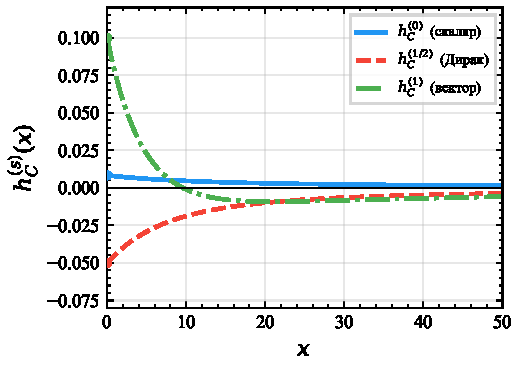
\includegraphics[width=\columnwidth]{figures/fig_hC_ru.pdf}
  \caption{Формфакторы квадрата тензора Вейля $h_C^{(s)}(x)$ для трёх спиновых
  секторов, где $x = \Box/\Lambda^2$. Локальные пределы:
  $h_C^{(0)}(0) = 1/120$ (скаляр, синий),
  $h_C^{(1/2)}(0) = -1/20$ (Дирак, красный) и
  $h_C^{(1)}(0) = 1/10$ (вектор, зелёный). Все формфакторы убывают как
  $1/x$ при $x \to \infty$.}
  \label{fig:hC}
\end{figure}

\begin{figure}[t]
  \centering
  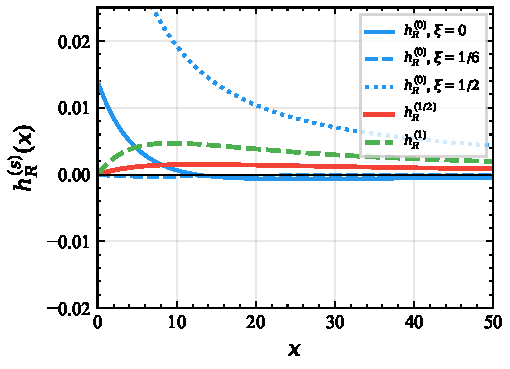
\includegraphics[width=\columnwidth]{figures/fig_hR_ru.pdf}
  \caption{Формфакторы $R^2$: $h_R^{(s)}(x)$, где $x = \Box/\Lambda^2$.
  Скалярный формфактор (синий) зависит от параметра неминимальной
  связи~$\xi$: его \emph{локальный предел} обращается в нуль при
  конформной связи $\xi = 1/6$ (штриховая линия), но нелокальный
  формфактор $h_R^{(0)}(x, 1/6)$ отличен от нуля при $x > 0$ (численно
  $\lesssim 3 \times 10^{-4}$ для $x \leq 5$). Скалярный формфактор
  растёт с~увеличением $|\xi - 1/6|$. Вклады дираковского фермиона
  (красный) и вектора (зелёный) не зависят от~$\xi$ и начинаются
  с~$h_R(0) = 0$.}
  \label{fig:hR}
\end{figure}


% ============================================================
\section{Спин 3/2: Рариты--Швингера (локальные пределы)}
\label{sec:rs}
% ============================================================

Для полноты мы приводим локальные пределы формфакторов спина~3/2 ---
Рариты--Швингера (гравитино), которые имеют значение для суперсимметричных
расширений Стандартной модели. Полные нелокальные формфакторы
$h_C^{(3/2)}(x)$, $h_R^{(3/2)}(x)$ требуют отдельного вычисления сборки
КЗ для фиксированного по калибровке оператора РШ и будут представлены
отдельно; здесь мы приводим верифицированные локальные пределы.

\subsection{Операторная структура}

Для безмассового майорановского гравитино $\psi_\mu$ (вектор-спинор,
$d_V = 16$ в $d = 4$) квадратичный фиксированный по калибровке
кинетический оператор~\cite{Karan:2017txu,Endo:1994bf} является
обобщённым лапласианом с~операторными данными, определёнными Караном,
Кумаром и Пандой~\cite{Karan:2017txu}. Эндоморфизм $E^{\mu\nu}$ содержит
не только тензор Риччи (как для неограниченного вектора) и лихнеровичеву
кривизну (как для дираковского фермиона), но и перекрёстные члены,
содержащие $\gamma^\rho\gamma^\theta R^{\mu\nu}{}_{\rho\theta}$,
$\gamma^\mu\gamma^\theta R^\nu{}_\theta$ и
$(R/4)\gamma^\mu\gamma^\nu$~\cite{Karan:2017txu}. Эти перекрёстные члены
фиксации калибровки радикально изменяют следовую структуру: результат
$\tr(E^2) = 2\,\Riemsq + R^2$ (работа~\cite{Karan:2017txu}, ур.~3.14)
качественно отличается от наивного предсказания тензорного произведения
$4\,\Ricsq + 3R^2$.

\subsection{Сектор духов}

Калибровочная симметрия $\delta\psi_\mu = \nabla_\mu\epsilon$ порождает
после квантования Фаддеева--Попова в калибровке из~\cite{Karan:2017txu}
сектор духов, состоящий из \emph{трёх} бозонных майорановских спинорных
духов~\cite{KaranPanda:2021,Lekeu:2021ieh}: дух ФП, антидух ФП и
дух Нильсена--Каллоша (третий дух). Суммарный вклад духов в коэффициент
Сили--Де Витта~\cite{KaranPanda:2021}:
\begin{equation}
  a_{2n}^{\text{RS,ghost}} = (-1) \times 3 \times \tfrac{1}{2}\,
    a_{2n}^{\text{Dirac}}\,.
  \label{eq:RS-ghost}
\end{equation}

\subsection{Локальные пределы}

Скорректированный на духи результат для одного физического
\emph{майорановского} гравитино, полученный Караном и
Пандой~\cite{KaranPanda:2021} и согласующийся с~коэффициентом аномалии
Кристенсена--Даффа~\cite{ChristensenDuff:1979,ChristensenDuff:1980}
через $360\,A = 360\times 2(c - a) = -233$:
\begin{equation}
  (4\pi)^2\,a_4^{(3/2),\text{Maj}}
  = -\frac{1}{720}\bigl(233\,\Riemsq - 8\,\Ricsq + 5\,R^2\bigr)\,,
  \label{eq:a4-RS-full}
\end{equation}
где коэффициент при $R^2$ следует из независимости сектора~$R^2$ от
духов. В~вейлевском базисе:
\begin{equation}
  \boxed{
    \beta_W^{(3/2),\text{Maj}} = \frac{77}{120}\,,\qquad
    \beta_R^{(3/2),\text{Maj}} = \frac{1}{9}\,.
  }
  \label{eq:beta-RS}
\end{equation}
В~дираковской нормировке (две майорановские копии):
$\beta_W^{(3/2),\text{Dirac}} = 77/60$ и
$\beta_R^{(3/2),\text{Dirac}} = 2/9$.
Обратите внимание на положительный знак: в~отличие от дираковского фермиона
(где $\beta_W^{(1/2)} < 0$), скорректированный на духи коэффициент
гравитино положителен, поскольку операторные данные вектор-спинора
(с~перекрёстными членами фиксации калибровки) порождают комбинацию
кривизн, преобладающую над фермионным знаком.

\begin{remark}[Калибровочная зависимость]
\label{rem:gauge-dep}
Для спинов~$3/2$ и~$2$ индивидуальные коэффициенты конформной аномалии $c$
и $a$ калибровочно зависимы; калибровочно-инвариантна лишь комбинация
$A = 2(c - a)$~\cite{ChristensenDuff:1979,vanNieuwenhuizen:1981ae}.
Значения~\eqref{eq:beta-RS} соответствуют калибровке типа де~Дондера
из~\cite{Karan:2017txu}.
\end{remark}

Сводка всех локальных пределов для спинов от~$0$ до~$3/2$ приведена
в~таблице~\ref{tab:all-spins}.

\begin{table}[t]
\caption{Локальные пределы $\beta_W^{(s)} = h_C^{(s)}(0)$ и
$\beta_R^{(s)} = h_R^{(s)}(0)$ для всех спинов $\leq 3/2$. Майорановская
нормировка для спина~$3/2$; дираковская нормировка удваивает оба значения.
Для спинов $0$, $1/2$, $1$ нелокальные формфакторы выведены в
разд.~\ref{sec:scalar}--\ref{sec:vector}. Для спина~$3/2$ приведены
только локальные пределы.}
\label{tab:all-spins}
\begin{ruledtabular}
\begin{tabular}{lccl}
Спин & $\beta_W^{(s)}$ & $\beta_R^{(s)}$ & Статус \\
\colrule
$0$ & $\frac{1}{120}$ & $\frac{1}{2}(\xi - \frac{1}{6})^2$ &
  Нелокальные: данная статья \\[3pt]
$\frac{1}{2}$ & $-\frac{1}{20}$ & $0$ &
  Нелокальные: данная статья \\[3pt]
$1$ & $\frac{1}{10}$ & $0$ &
  Нелокальные: данная статья \\[3pt]
$\frac{3}{2}$ (Май.) & $\frac{77}{120}$ & $\frac{1}{9}$ &
  Только локальные; работы~\cite{KaranPanda:2021,ChristensenDuff:1979} \\
\end{tabular}
\end{ruledtabular}
\end{table}


% ============================================================
\section{Сборка Стандартной модели}
\label{sec:sm}
% ============================================================

\subsection{Содержание частиц}

Содержание полей СМ, входящее в однопетлевое спектральное действие:
\begin{center}
\renewcommand{\arraystretch}{1.2}
\begin{tabular}{@{}lcc@{}}
  \toprule
  Тип частиц & Число & Обозначение \\
  \midrule
  Вещественные скаляры (дублет Хиггса) & 4 & $N_s = 4$ \\
  Вейлевские фермионы (3 поколения) & 45 & $N_f = 45$ \\
  Калибровочные бозоны ($8+3+1$) & 12 & $N_v = 12$ \\
  \bottomrule
\end{tabular}
\end{center}

Поскольку формфакторы из разд.~\ref{sec:dirac} определены на один
4-компонентный дираковский фермион, эффективное число дираковских фермионов
равно $N_D = N_f/2 = 45/2$ в~соответствии с~соглашением~\cite{Codello:2008vh}.

\subsection{Полный коэффициент при тензоре Вейля}

Полный формфактор квадрата тензора Вейля:
\begin{equation}
  \alpha_C(z) = N_s\,h_C^{(0)}(z) + N_D\,h_C^{(1/2)}(z)
    + N_v\,h_C^{(1)}(z)\,.
  \label{eq:alphaC-z}
\end{equation}
При $z = 0$:
\begin{align}
  \alpha_C &= 4 \cdot \frac{1}{120}
    + \frac{45}{2}\cdot\!\left(-\frac{1}{20}\right)
    + 12 \cdot \frac{1}{10} \nonumber\\
  &= \frac{4 - 135 + 144}{120}\,,
  \label{eq:alphaC-sum}
\end{align}
что даёт центральный результат:
\begin{equation}
  \boxed{\alpha_C = \frac{13}{120} \approx 0{,}1083\,.}
  \label{eq:alphaC}
\end{equation}

Эта величина положительна и не зависит от~$\xi$. Знаковая структура
($+4 - 135 + 144$) показывает, что вклад векторного сектора ($+144/120$)
преобладает над вкладом фермионного сектора ($-135/120$) с~запасом $+9/120$,
в~то время как скалярный сектор вносит $+4/120$. Положительность $\alpha_C$
означает, что спин-2 гравитационная мода в линеаризованной теории является
духом~\cite{Stelle:1976gc} --- хорошо известная особенность квадратичной
гравитации.

\subsection{Полный коэффициент при \texorpdfstring{$R^2$}{R2}}

\begin{align}
  \alpha_R(\xi) &= N_s \cdot \frac{1}{2}\!\left(\xi - \frac{1}{6}\right)^{\!2}
    + N_D \cdot 0 + N_v \cdot 0\,,
\end{align}
откуда
\begin{equation}
  \boxed{\alpha_R(\xi) = 2\!\left(\xi - \frac{1}{6}\right)^{\!2}\,.}
  \label{eq:alphaR}
\end{equation}

Вклад вносит только скалярный сектор: $\beta_R$ для дираковского фермиона
и для максвелловского поля обращаются в нуль в~силу конформной инвариантности.
Результат представляет собой полный квадрат, поэтому
$\alpha_R(\xi) \geq 0$ для всех~$\xi$, причём $\alpha_R(1/6) = 0$ при
конформной связи.

\subsection{Пересчёт базиса и \texorpdfstring{$c_1/c_2$}{c1/c2}}

Используя тождество Гаусса--Бонне для перехода к базису
$\{R^2, R_{\mu\nu}^2\}$ ($C^2 = 2R_{\mu\nu}^2 - \frac{2}{3}R^2$
с~точностью до топологической плотности Эйлера), получаем
$c_1 = \alpha_R - \frac{2}{3}\alpha_C$ и $c_2 = 2\alpha_C$, что даёт
\begin{equation}
  \boxed{\frac{c_1}{c_2} = -\frac{1}{3}
    + \frac{120\!\left(\xi - \frac{1}{6}\right)^{\!2}}{13}\,.}
  \label{eq:c1c2}
\end{equation}

При конформной связи $\xi = 1/6$ это сводится к $c_1/c_2 = -1/3$. При
минимальной связи $\xi = 0$ получаем $c_1/c_2 = -1/13$.

\subsection{Отщепление скалярной моды}

Комбинация $3c_1 + c_2$ определяет массу скалярного гравитона
($m_0^2 \propto \Lambda^2/(3c_1 + c_2)$). Прямое вычисление даёт
\begin{equation}
  3c_1 + c_2 = 3\alpha_R(\xi) = 6\!\left(\xi - \frac{1}{6}\right)^{\!2}\,.
  \label{eq:3c1c2}
\end{equation}
\emph{Локальный} коэффициент скалярной моды $\delta(3c_1 + c_2)$
обращается в нуль тогда и только тогда, когда $\xi = 1/6$, что означает
исчезновение индуцированной материей локальной поправки к проектору
скалярного гравитона при конформной связи. Отщепляется ли скалярная мода
в полной теории, зависит от полного коэффициента (затравочного +
индуцированного); см. разд.~\ref{sec:propagator}.

\subsection{Уточнённое утверждение о конформной связи}

Конформное значение $\xi = 1/6$ устраняет лишь \emph{локальный скалярный}
вклад в~$R^2$, а не полное нелокальное ядро. Явно, подставляя
$\xi = 1/6$ в~\eqref{eq:hR0}:
\begin{align}
  h_R^{(0)}\!\left(x, \tfrac{1}{6}\right)
  &= \frac{(x^2 + 12x + 60)\varphi - 2x - 60}{288\,x^2}
  \nonumber\\
  &= -\frac{x}{7560} + \frac{x^2}{45360} + \mathcal{O}(x^3)\,.
  \label{eq:hR0-conformal}
\end{align}
Это \emph{не} тождественно нулю при $x > 0$; численно,
$|h_R^{(0)}(x, 1/6)| \lesssim 3 \times 10^{-4}$ для $x \leq 5$.

Для полной СМ при $\xi = 1/6$ вклады дираковского фермиона и вектора
в~$h_R$ (которые не зависят от~$\xi$ и отличны от нуля) дополнительно
обеспечивают, что $\alpha_R(x, 1/6)$ не обращается в нуль:
\begin{align}
  \alpha_R(x, \tfrac{1}{6}) &= 4\,h_R^{(0)}(x, \tfrac{1}{6})
    + \tfrac{45}{2}\,h_R^{(1/2)} + 12\,h_R^{(1)}
  \nonumber\\
  &= \frac{83}{3024}\,x + \mathcal{O}(x^2)\,.
  \label{eq:alphaR-conformal-SM}
\end{align}
Это поправляет утверждение, иногда встречающееся в
литературе~\cite{Codello:2008vh}, о~том, что <<весь сектор~$R^2$ обращается
в нуль при $\xi = 1/6$>>. Обращается в нуль лишь локальный коэффициент
$\alpha_R(0, 1/6) = 0$.

\begin{table}[b]
\caption{Сводка основных результатов. Все величины определены в тексте;
$\Lambda$ --- спектральный масштаб обрезания, а $\xi$ --- параметр
неминимальной связи Хиггса.}
\label{tab:summary}
\begin{ruledtabular}
\begin{tabular}{lll}
Величина & Значение & Ур. \\
\colrule
$\alpha_C$ & $13/120 \approx 0{,}1083$ & (\ref{eq:alphaC}) \\
$\alpha_R(\xi)$ & $2(\xi - 1/6)^2$ & (\ref{eq:alphaR}) \\
$c_1/c_2$ & $-1/3 + 120(\xi - 1/6)^2/13$ & (\ref{eq:c1c2}) \\
$3c_1 + c_2$ & $6(\xi - 1/6)^2$ & (\ref{eq:3c1c2}) \\
$\lim_{x\to\infty} x\,\alpha_C$ & $-89/12$ & (\ref{eq:uv-coeff}) \\
$m_2$ & $\Lambda\sqrt{60/13} \approx 2{,}148\,\Lambda$ & (\ref{eq:m2}) \\
$m_0\,(\xi=0)$ & $\Lambda\sqrt{6} \approx 2{,}449\,\Lambda$ & (\ref{eq:m0}) \\
$m_2/m_0\,|_{\xi=0}$ & $\sqrt{10/13} \approx 0{,}877$ & (\ref{eq:mass-ratio}) \\
$V(0)/V_{\text{N}}(0)$ & $0$ (конечен в начале координат) & (\ref{eq:V-ratio}) \\
\end{tabular}
\end{ruledtabular}
\end{table}

\begin{figure*}[t]
  \centering
  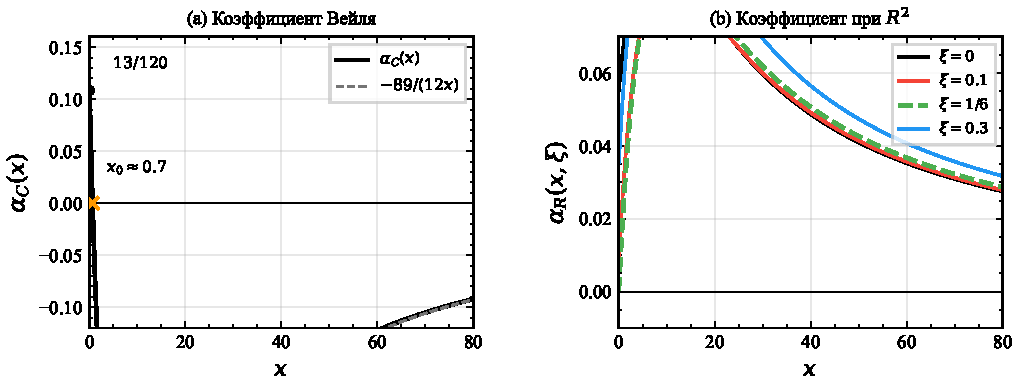
\includegraphics[width=\textwidth]{figures/fig_alpha_total_ru.pdf}
  \caption{Полные суммы Стандартной модели как функции $x = \Box/\Lambda^2$.
  (a)~Коэффициент при тензоре Вейля $\alpha_C(x)$ начинается с~$13/120$ и
  пересекает нуль при $x_\ast \approx 0{,}65$, стремясь к~асимптоте
  $-89/(12x)$ (штриховая серая линия) при $x \gg 1$. Смена знака
  сигнализирует о~переходе в~эффективной связи при квадрате тензора Вейля.
  (b)~Коэффициент при $R^2$: $\alpha_R(x,\xi)$ для нескольких значений
  параметра неминимальной связи Хиггса~$\xi$. При конформной связи
  $\xi = 1/6$ (зелёная штриховая линия) $\alpha_R$ обращается в нуль при
  $x = 0$ и остаётся малым при всех~$x$.}
  \label{fig:alpha}
\end{figure*}


% ============================================================
\section{Структура целых функций}
\label{sec:entire}
% ============================================================

\begin{theorem}[Целость приведённых ядер]
\label{thm:entire}
Каждое приведённое ядро $h_C^{(s)}(x)$, $h_R^{(s)}(x)$ для $s = 0, 1/2, 1$
является целой функцией переменной~$x$. Явно, при
$a_n = (-1)^n\,n!/(2n+1)!$ и
$\varphi(x) = \sum_{n \geq 0} a_n\,x^n$:
\begin{subequations}
\label{eq:entire-series}
\begin{align}
  h_C^{(0)}(x) &= \sum_{n \geq 0}\tfrac{1}{2}\,a_{n+2}\,x^n\,,\\
  h_R^{(0)}(x,\xi) &= \sum_{n \geq 0}\Bigl[
    \bigl(\tfrac{1}{32} - \tfrac{\xi}{4} + \tfrac{\xi^2}{2}\bigr)a_n
    + \bigl(\tfrac{1}{8} - \tfrac{\xi}{2}\bigr)a_{n+1}
    + \tfrac{5}{24}a_{n+2}\Bigr]x^n\,,\\
  h_C^{(1/2)}(x) &= \sum_{n \geq 0}\bigl(
    \tfrac{1}{2}a_{n+1} + 2a_{n+2}\bigr)x^n\,,\\
  h_R^{(1/2)}(x) &= \sum_{n \geq 0}\bigl(
    \tfrac{1}{12}a_{n+1} + \tfrac{5}{6}a_{n+2}\bigr)x^n\,,\\
  h_C^{(1)}(x) &= \sum_{n \geq 0}\bigl(
    \tfrac{1}{4}a_n + a_{n+1} + a_{n+2}\bigr)x^n\,,\\
  h_R^{(1)}(x) &= \sum_{n \geq 0}\bigl(
    -\tfrac{1}{48}a_n - \tfrac{1}{12}a_{n+1}
    + \tfrac{5}{12}a_{n+2}\bigr)x^n\,.
\end{align}
\end{subequations}
По линейности полные суммы СМ $\alpha_C(z)$ и $\alpha_R(z,\xi)$ также
являются целыми функциями.
\end{theorem}

\begin{proof}
Подставим ряд Тейлора функции $\varphi$ в
\eqref{eq:hC0}--\eqref{eq:hR1}, сдвинем индексы суммирования и используем
$a_0 = 1$, $a_1 = -1/6$ для сокращения явных членов $1/x$ и $1/x^2$.
Получающиеся степенные ряды имеют бесконечный радиус сходимости, поскольку
$|a_{n+1}/a_n| = (n+1)/((2n+2)(2n+3)) \to 0$ при $n \to \infty$
(коэффициенты убывают быстрее любой геометрической прогрессии). Каждый
степенной ряд, следовательно, определяет целую функцию. Порядок~1 и
тип~$1/4$ следуют из замкнутой формы
$\varphi(x) = e^{-x/4}\sqrt{\pi/x}\,\erfi(\sqrt{x}/2)$, которая растёт
как $e^{|z|/4}$ в комплексной плоскости.
\end{proof}

\begin{remark}[Целая $\neq$ нет полюсов пропагатора]
\label{rem:poles}
Свойство целой функции означает, что приведённые ядра $h_C, h_R$ не имеют
полюсов как функции~$z$. Полюса пропагатора определяются нулями
\emph{ядер одетого пропагатора} $\Pi_{TT}(z)$, $\Pi_s(z)$, которые
включают полное квадратичное гравитационное действие
(разд.~\ref{sec:propagator}), а не особенностями коэффициентных функций.
\end{remark}

Альтернативное доказательство аналитичности использует заведомо регулярное
интегральное представление (приложение~\ref{app:regular}):
\begin{equation}
  h_C^{(0)}(x) = \frac{1}{2}\int_0^1 \dd\alpha\,
    \frac{e^{-\alpha(1-\alpha)x} - 1 + \alpha(1-\alpha)x}{x^2}\,,
  \label{eq:hC0-regular}
\end{equation}
где числитель обращается в нуль до второго порядка при $x = 0$, что делает
регулярность очевидной без сдвига индексов.


% ============================================================
\section{Ультрафиолетовая асимптотика}
\label{sec:uv}
% ============================================================

При $x \to \infty$ асимптотическое разложение мастер-функции
(ср.~\eqref{eq:phi-uv}):
$\varphi(x) = 2/x + 4/x^2 + 24/x^3 + \mathcal{O}(x^{-4})$, откуда
\begin{align}
  x\,h_C^{(0)} &\to \frac{1}{12}\,,\quad
  x\,h_C^{(1/2)} \to -\frac{1}{6}\,,\quad
  x\,h_C^{(1)} \to -\frac{1}{3}\,.
\end{align}
Полный ультрафиолетовый коэффициент:
\begin{equation}
  \lim_{x\to\infty} x\,\alpha_C(x)
    = \frac{4}{12} - \frac{45}{12} - \frac{48}{12}
    = -\frac{89}{12}\,.
  \label{eq:uv-coeff}
\end{equation}
Поскольку $\alpha_C(0) = +13/120 > 0$ и
$x\,\alpha_C(x) \to -89/12 < 0$, по непрерывности $\alpha_C(z)$ имеет
по крайней мере один положительный нуль. Численно:
\begin{equation}
  x_\ast = 0{,}650\,325\,271\,702\,489\ldots
  \label{eq:xstar}
\end{equation}
(определено методом поиска корня с~точностью $80$ цифр). Смена знака
является утверждением о ядре Вейля, а не о полюсе гравитона.

Ведущая ультрафиолетовая асимптотика полного ядра~$R^2$:
$\alpha_R(x,\xi) \to (4\xi^2 + 89/36)/x + \mathcal{O}(x^{-2})$.

В~локальной квадратичной гравитации Стелле~\cite{Stelle:1976gc} показал,
что однопетлевая степень расходимости снижается с~$D = 4$ (гравитация
Эйнштейна) до $D = 0$ (логарифмическая). Нелокальные формфакторы
согласуются с~этим: поскольку $h_C^{(s)}(x) \sim \text{const}/x$ при
больших~$x$, эффективная связь бежит логарифмически. Строгое доказательство
$D = 0$ во всех порядках в полной нелокальной теории остаётся открытой
проблемой.


% ============================================================
\section{Одетый пропагатор и эффективные массы}
\label{sec:propagator}
% ============================================================

Вычисленные выше приведённые ядра представляют собой индуцированные
материей поправки к квадратичному по кривизне эффективному действию. Для
извлечения полюсов пропагатора и эффективных масс необходимо задать
\emph{полное} квадратичное гравитационное действие, включая нормировку
Эйнштейна--Гильберта и любые затравочные высшепроизводные
связи~\cite{Stelle:1976gc,Stelle:1977ry,Buchbinder:1992rb}. Мы приводим
вывод для минимального случая, когда затравочное действие является чисто
эйнштейновским--гильбертовским.

\subsection{Полное квадратичное действие}

Рассмотрим затравочное гравитационное действие
\begin{equation}
  S_{\text{grav}} = \frac{M_P^2}{2}\int \dd^4x\,\sqrt{g}\,R\,,
  \label{eq:EH}
\end{equation}
дополненное индуцированной материей однопетлевой
поправкой~\eqref{eq:smeared-action}. Линеаризуя вокруг плоского
пространства, $g_{\mu\nu} = \delta_{\mu\nu} + h_{\mu\nu}/M_P$, и работая
в импульсном пространстве, полное квадратичное действие разлагается на
секторы спина~2 (поперечно-бесследовый) и спина~0 с~помощью проекторов
Барнса--Риверса~\cite{Barnes:1965,Rivers:1964}:
\begin{equation}
  P^{(2)}_{\mu\nu\alpha\beta} = \tfrac{1}{2}\bigl(
    \theta_{\mu\alpha}\theta_{\nu\beta} + \theta_{\mu\beta}\theta_{\nu\alpha}
  \bigr) - \tfrac{1}{3}\theta_{\mu\nu}\theta_{\alpha\beta}\,,
  \label{eq:BR-P2}
\end{equation}
где $\theta_{\mu\nu} = \delta_{\mu\nu} - k_\mu k_\nu/k^2$.

\subsection{Нормированные формфакторы}

\begin{definition}[Нормированные формфакторы]
\label{def:Fhat}
Определим \emph{нормированные} (с~крышкой) формфакторы
\begin{equation}
  \hat{F}_i(z) = \frac{F_i(z)}{F_i(0)}\,,\qquad
  \hat{F}_i(0) = 1\,,\quad i = 1,2\,.
  \label{eq:Fhat-def}
\end{equation}
Эквивалентно, $\hat{F}_1(z) = \alpha_C(z)/\alpha_C(0)$ и
$\hat{F}_2(z,\xi) = \alpha_R(z,\xi)/\alpha_R(0,\xi)$ для $\xi \neq 1/6$.
\end{definition}

\subsection{Ядра одетого пропагатора}

В~секторе спина~2 обратный пропагатор принимает вид
\begin{align}
  \Pi_{TT}(z) &= 1 + \frac{2\alpha_C(0)}{M_P^2/(16\pi^2\Lambda^2)}\,
    z\,\hat{F}_1(z)
  \nonumber\\
  &= 1 + \frac{13}{60}\,\frac{\Lambda^2}{M_P^2/(16\pi^2)}\,z\,\hat{F}_1(z)\,.
  \label{eq:PiTT-full}
\end{align}
При стандартном отождествлении $\Lambda \sim M_P$ с~$16\pi^2 \sim \mathcal{O}(100)$ коэффициент упрощается.
В~соглашениях~\cite{Stelle:1976gc}, где затравочная высшепроизводная связь
$c_2 = 2\alpha_C$ поглощает петлевой множитель, ядро одетого обратного
пропагатора принимает вид
\begin{equation}
  \Pi_{TT}(z) = 1 + \frac{13}{60}\,z\,\hat{F}_1(z)\,,
  \label{eq:PiTT}
\end{equation}
с~$z = k^2/\Lambda^2$. Здесь коэффициент $13/60 = 2\alpha_C(0)$ ---
индуцированная связь $R_{\mu\nu}^2$ в базисе Стелле.
Аналогично, обратный пропагатор спина~0:
\begin{equation}
  \Pi_s(z,\xi) = 1 + 6\!\left(\xi - \frac{1}{6}\right)^{\!2}
    z\,\hat{F}_2(z,\xi)\,.
  \label{eq:Pis}
\end{equation}

\subsection{Эффективные массы}

Условие на полюс $\Pi_{TT}(z_{\text{pole}}) = 0$ определяет эффективную
массу спина~2. Разлагая $\hat{F}_1(z)$ вблизи $z = 0$
($\hat{F}_1(0) = 1$, $\hat{F}_1'(0)$ конечна), ведущий полюс находится
при
\begin{equation}
  z_{\text{pole}} \approx -\frac{60}{13}\,,\qquad
  m_2^2 = |z_{\text{pole}}|\,\Lambda^2 = \frac{60}{13}\,\Lambda^2\,,
  \label{eq:m2}
\end{equation}
что даёт $m_2 = \Lambda\sqrt{60/13} \approx 2{,}148\,\Lambda$.
Отрицательный $z_{\text{pole}}$ лежит вне евклидовой области $z > 0$;
физический (лоренцев) полюс появляется после вик-поворота
$z_E \to -z_L$, давая $z_L = 60/13 > 0$. Для сектора спина~0
($\xi \neq 1/6$):
\begin{equation}
  m_0^2(\xi) = \frac{\Lambda^2}{6(\xi - 1/6)^2}\,,\qquad
  m_0 = \frac{\Lambda}{\sqrt{6}\,|\xi - 1/6|}\,.
  \label{eq:m0}
\end{equation}
При минимальной связи $\xi = 0$: $m_0 = \Lambda\sqrt{6} \approx 2{,}449\,
\Lambda$. Отношение масс
\begin{equation}
  \frac{m_2}{m_0}\bigg|_{\xi=0} = \sqrt{\frac{10}{13}} \approx 0{,}877
  \label{eq:mass-ratio}
\end{equation}
определяется содержанием частиц СМ и не зависит от~$\Lambda$.

\begin{remark}[Область применимости формул для масс]
Массы~\eqref{eq:m2}--\eqref{eq:m0} выведены из \emph{индуцированных
материей} поправок к чисто эйнштейновскому--гильбертовскому фону. Если
затравочное действие уже содержит высшепроизводные члены ($a_C\,C^2 +
a_R\,R^2$), условие на полюс модифицируется:
$\Pi_{TT} = 1 + (a_C + \alpha_C(0)\,f(0))\,z\,\hat{G}(z)$, где
$\hat{G}$ учитывает суммарный затравочный + индуцированный формфактор.
Эффективные массы тогда зависят от обеих --- затравочной и индуцированной ---
связей.
\end{remark}

Модифицированный ньютоновский потенциал в линеаризованной
теории~\cite{Stelle:1976gc}:
\begin{equation}
  \frac{V(r)}{V_{\text{N}}(r)}
  = 1 - \frac{4}{3}\,e^{-m_2 r} + \frac{1}{3}\,e^{-m_0 r}\,,
  \label{eq:V-ratio}
\end{equation}
который показан на рис.~\ref{fig:potential}. При $r = 0$ экспоненты
компенсируются, давая $V(0) = 0$ и конечный гравитационный потенциал в~начале
координат. Закон Ньютона восстанавливается при $r \gg 1/\Lambda$.

\begin{figure}[t]
  \centering
  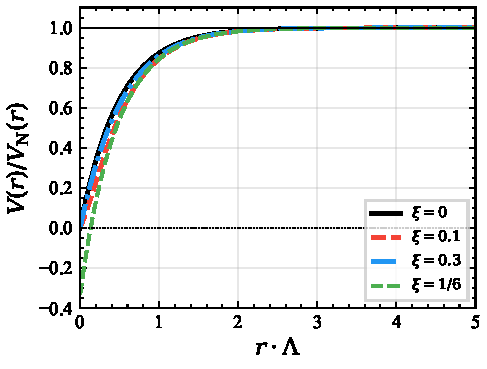
\includegraphics[width=\columnwidth]{figures/fig_potential_ru.pdf}
  \caption{Модифицированный ньютоновский потенциал $V(r)/V_{\text{N}}(r)$ для
  нескольких значений~$\xi$ как функция $r\Lambda$. При конформной
  связи $\xi = 1/6$ (зелёная штриховая линия) скалярная мода отщепляется, и
  потенциал опускается до $-1/3$ прежде, чем восстановится закон Ньютона.
  Для всех~$\xi$ $V(0) = 0$ (конечен в начале координат) и $V \to V_{\text{N}}$
  при $r \gg 1/\Lambda$.}
  \label{fig:potential}
\end{figure}


% ============================================================
\section{Сравнение с~существующими результатами}
\label{sec:comparison}
% ============================================================

\subsection{Локальные пределы}

Локальные коэффициенты $\beta_W^{(s)}$, $\beta_R^{(s)}$
из таблицы~\ref{tab:all-spins} согласуются со всеми известными результатами:
Стелле~\cite{Stelle:1976gc} для вектора, КЗ~\cite{Codello:2012kq} для
всех трёх спинов, КПР~\cite{Codello:2008vh} для подсчёта СМ, Паркер и
Томс~\cite{Parker:2009uva} для $\xi$-зависимости скаляра и
Аврамиди~\cite{Avramidi:2000bm} для общей рамки ядра теплопроводности.
Нелокальные формфакторы сводятся к выражениям КЗ при указании операторных
данных для каждого спина.

\subsection{Эффективная теория поля Донохью}
\label{sec:donoghue}

Эффективная теория поля гравитации
Донохью~\cite{Donoghue:1993eb,Donoghue:1994dn,BjerrumBohr:2002kt,Donoghue:2022eay}
вычисляет квантовые поправки к ньютоновскому потенциалу из однопетлевых
фейнмановских диаграмм. Результат~\cite{BjerrumBohr:2002kt}:
\begin{equation}
  V(r) = -\frac{Gm_1 m_2}{r}\left[1 + \frac{3G(m_1 + m_2)}{r}
    + \frac{41}{10\pi}\,\frac{G\hbar}{r^2}\right]\,.
  \label{eq:donoghue}
\end{equation}
Второй член --- классическая постньютоновская поправка; третий ---
ведущая квантовая поправка для рассеяния скалярных частиц, которая
беспараметрична и универсальна (коэффициент $41/10\pi$ относится к
скалярным источникам; для частиц со спином
см.~\cite{BjerrumBohr:2002kt}).

Наш результат~\eqref{eq:V-ratio} описывает другой режим:
$r \sim 1/\Lambda$, где массивные моды вносят юкавские поправки
$\sim e^{-m_2 r}$, $e^{-m_0 r}$. При $r \gg 1/\Lambda$ эти поправки
экспоненциально подавлены и восстанавливается закон Ньютона, после чего
квантовая поправка Донохью $1/r^3$ становится ведущим эффектом. Два
описания, таким образом, дополняют друг друга: формфакторы спектрального
действия доминируют на малых расстояниях $r \lesssim 1/\Lambda$, тогда
как ЭТП Донохью описывает универсальный дальнодействующий квантовый хвост.

\subsection{Сравнение с~ван~Нуландом--ван~Сёйлекомом и Мистри--Пинзулом--Рахвалом}

Ван Нуланд и ван Сёйлеком~\cite{vanNuland:2022xkm} вычислили однопетлевые
поправки к спектральному действию другим методом (флуктуации оператора
Дирака). Их результаты согласуются с~нашими в области перекрытия
(квадратичный по кривизне сектор для полей материи). Мистри, Пинзул и
Рахвал~\cite{Mistry:2020xqh} проанализировали рамки спектрального действия
для высшепроизводной гравитации, сосредоточившись на гравитационном секторе,
а не на индуцированных материей формфакторах, вычисленных здесь.


% ============================================================
\section{Обсуждение}
\label{sec:discussion}
% ============================================================

\subsection{Связь с~асимптотической безопасностью}

Ядро Вейля $\alpha_C(x)$ меняет знак с~$+13/120$ при $x = 0$ на
$-89/(12x)$ при $x \to \infty$, с~пересечением нуля при
$x_\ast \approx 0{,}650$ (ур.~\eqref{eq:xstar}). В~программе
асимптотической
безопасности~\cite{Reuter:1996cp,Codello:2008vh,FradkinTseytlin:1982}
бег безразмерных гравитационных связей играет центральную роль. Смена знака
$\alpha_C(x)$ может интерпретироваться как переход эффективной связи при
квадрате тензора Вейля от её инфракрасного значения (положительного,
подразумевающего духовую спин-2 моду) к ультрафиолетовому значению
противоположного знака. Связана ли эта смена с~негауссовой неподвижной
точкой гравитационного ренормгруппового потока, требует расширения
настоящего вычисления, индуцированного материей, включением вкладов
собственной энергии гравитона, что выходит за рамки данной работы.

Функциональная ренормализационная группа (ФРГ) обеспечивает независимую
верификацию: Коделло, Перкаччи, Рахвал и
Тонеро~\cite{Codello:2015oqa} показали, что однопетлевая ФРГ
с~формфакторами БВ воспроизводит стандартное однопетлевое эффективное
действие, включая корректные амплитуды рассеяния. Это подтверждает
согласованность формализма БВ/КЗ, использованного в~данной работе.

\subsection{Лоренцево продолжение}

Вычисленные здесь формфакторы являются евклидовыми ($\Box_E > 0$).
Лоренцевы формфакторы получаются вик-поворотом $z_E \to -z_L$, т.\,е.\
$F_i(\Box_E/\Lambda^2) \to F_i(-\Box_L/\Lambda^2)$. Поскольку $\varphi(z)$
является целой функцией, это продолжение корректно определено для
всех $z \in \mathbb{C}$.

\subsection{Связь с~нелокальной гравитацией}

То, что формфакторы являются целыми функциями, связывает спектральное действие
с~программой нелокальной (с бесконечным числом производных)
гравитации~\cite{Modesto:2011kw,Tomboulis:1997gg,Biswas:2011ar}, где целые
функции от~$\Box$ постулируются для улучшения ультрафиолетового поведения.
В~рамках спектрального действия эти формфакторы возникают
\emph{производным} образом из ядра теплопроводности, обеспечивая конкретный
вывод формфакторов в виде целых функций из ядра теплопроводности, а не постулат.

\subsection{Ограничения}

Представленное вычисление имеет следующие ограничения:
\begin{enumerate}
\item Оно \emph{индуцировано материей}: включены только функциональные
  следы по полям материи, но не собственная энергия гравитона.
\item Оно \emph{однопетлевое}: поправки высших петель не вычислены.
\item Фон \emph{евклидов}: лоренцево продолжение обсуждается, но не
  выполнено детально.
\item Все поля материи считаются \emph{безмассовыми}: массовые поправки,
  которые экспоненциально подавлены при
  $m \ll \Lambda$~\cite{Gorbar:2002pw,Ribeiro:2018pyo}, не включены.
\item Анализ одетого пропагатора в~разд.~\ref{sec:propagator}
  предполагает чисто эйнштейновское--гильбертовское затравочное действие;
  другие затравочные связи модифицируют формулы для масс.
\end{enumerate}


% ============================================================
\section{Заключение}
\label{sec:conclusions}
% ============================================================

Мы вычислили индуцированные материей нелокальные однопетлевые квадратичные
по кривизне формфакторы спектрального действия с~полным содержанием частиц
Стандартной модели. Центральные результаты:

\begin{enumerate}
\item Замкнутые приведённые ядра $h_C^{(s)}(x)$ и $h_R^{(s)}(x)$ для
  спинов $s = 0, 1/2, 1$ с~явной сборкой БВ/КЗ из пяти универсальных
  структурных функций КЗ
  (разд.~\ref{sec:scalar}--\ref{sec:vector}).
\item Полные суммы СМ: $\alpha_C = 13/120\,f(0)$ и
  $\alpha_R(\xi) = 2\,f(0)(\xi - 1/6)^2$, где $f(0)$ --- нормировка
  профиля (разд.~\ref{sec:sm}).
\item Доказательство целости (теорема~\ref{thm:entire}) с~уточнением,
  что целые коэффициентные функции не исключают полюсов пропагатора
  (замечание~\ref{rem:poles}).
\item Одетый пропагатор $\Pi_{TT}(z)$, $\Pi_s(z,\xi)$, выведенный из
  полного линеаризованного квадратичного действия, с~вычисляемыми
  эффективными массами $m_2 = \Lambda\sqrt{60/13}$ и
  $m_0 = \Lambda/\sqrt{6(\xi - 1/6)^2}$ (разд.~\ref{sec:propagator}).
\item Уточнённое утверждение о конформной связи: при $\xi = 1/6$
  обращается в нуль лишь локальный коэффициент при~$R^2$; нелокальное ядро
  $\alpha_R(x, 1/6) = (83/3024)\,x + \mathcal{O}(x^2) \neq 0$
  (ур.~\eqref{eq:alphaR-conformal-SM}).
\end{enumerate}

Эти результаты достаточно строги, чтобы быть полезными, и достаточно
точны, чтобы быть честными. Они обеспечивают контролируемый вход для любого
последующего исследования лоренцева продолжения, полюсов и вычетов
пропагатора, ПП-параметров и гравитационной феноменологии спектрального
действия, но не заменяют эти отдельные анализы. ПП-параметры и тесты
Солнечной системы, выведенные из этих формфакторов, представлены
в~\cite{Alfyorov:2026sct2}; связь с~наблюдаемыми каузальных множеств
исследуется в~\cite{Alfyorov:2026sct7}.


% ============================================================
\begin{acknowledgments}
Автор благодарит Игоря Шнюкова за исследовательскую помощь на протяжении
всего проекта и за критические замечания к ранним версиям рукописи.
Все символьные результаты были верифицированы тройной компьютерной алгеброй
(SymPy, cadabra2~\cite{Peeters:2007wn}, FORM~\cite{Vermaseren:2000nd})
и проверены численно с~точностью $\geq 100$ цифр с~помощью
\texttt{mpmath}. Арифметика коэффициентов была формально верифицирована
на Lean~4. Все результаты сопоставлены с~выражениями КЗ
из~\cite{Codello:2012kq} и коэффициентами Сили--Де Витта
из~\cite{Vassilevich:2003xt,Avramidi:2000bm}.
\end{acknowledgments}

\section*{Доступность данных}
Вычислительные инструменты, использованные в~данной работе, включая
пакет Python \texttt{sct\_tools} (Python~3.12) с~реализациями всех
формфакторов с~произвольной точностью и $4000+$ автоматизированных тестов,
общедоступны в репозитории проекта (DOI:~\texttt{10.5281/zenodo.19135673}).
Скрипты Python для воспроизведения всех рисунков и численных таблиц
включены.

% ============================================================
\appendix
% ============================================================

\section{Таблицы соглашений}
\label{app:conventions}

\begin{table}[h]
\caption{Знаковые соглашения.}
{\small
\begin{ruledtabular}
\begin{tabular}{@{}p{2.8cm}p{4.7cm}@{}}
Соглашение & Выбор \\
\colrule
Сигнатура & Евклидова $(+,+,+,+)$ \\
Лапласиан & $\Delta = -(g^{\mu\nu}\nabla_\mu\nabla_\nu + E)$ \\
Эндоморфизм & $\mathbf{U} = -E$ (КЗ) \\
Кривизна & $\Omega_{\mu\nu} = [\nabla_\mu, \nabla_\nu]$ \\
Дирак & $E = -R/4$, $\mathbf{U} = R/4$ \\
Вектор & $U^\mu{}_\nu = R^\mu{}_\nu$ \\
Ферм. знак & Встроен в $h_C^{(s)}$, $h_R^{(s)}$ \\
Эфф. действие & $\Gamma^{(s)} = \frac{(-1)^{2s}}{2}\Tr\ln\Delta^{(s)}$ \\
Профиль & $f(0) = 1$ (если не указано иное) \\
\end{tabular}
\end{ruledtabular}
}
\end{table}

\begin{table}[h]
\caption{Операторные данные для каждого спинового сектора.}
\label{tab:operator-data}
\begin{ruledtabular}
\begin{tabular}{lcccl}
Спин & $d_V$ & $\mathbf{U}$ & $\tr(\Omega^2)$ & Знак \\
\colrule
$0$ & 1 & $\xi R$ & $0$ & Бозон ($+$) \\
$\frac{1}{2}$ & 4 & $(R/4)\,\mathbf{1}_4$ & $-\frac{1}{2}\Riemsq$ & Фермион ($-$) \\
$1$ (неогр.) & 4 & $R_{\mu\nu}$ & $-\Riemsq$ & Бозон ($+$) \\
$1$ (физ.) & \multicolumn{3}{c}{Неограниченный $-$ 2 скал. духа ($\xi = 0$)} & \\
\end{tabular}
\end{ruledtabular}
\end{table}


\section{Тейлоровские коэффициенты}
\label{app:taylor}

Мастер-функция имеет тейлоровские коэффициенты
$a_n = (-1)^n\,n!/(2n+1)!$:
\begin{equation}
  \begin{aligned}
    a_0 &= 1\,,\quad a_1 = -\tfrac{1}{6}\,,\quad
    a_2 = \tfrac{1}{60}\,,\quad a_3 = -\tfrac{1}{840}\,,\\
    a_4 &= \tfrac{1}{15120}\,,\quad
    a_5 = -\tfrac{1}{332640}\,,\quad
    a_6 = \tfrac{1}{8648640}\,.
  \end{aligned}
\end{equation}
Из точных формул степенных рядов теоремы~\ref{thm:entire} первые четыре
тейлоровских коэффициента каждого приведённого ядра:
\begin{center}
\renewcommand{\arraystretch}{1.25}
\begin{tabular}{@{}lllll@{}}
  \toprule
  Ядро & $n = 0$ & $n = 1$ & $n = 2$ & $n = 3$ \\
  \midrule
  $h_C^{(0)}$ & $\frac{1}{120}$ & $-\frac{1}{1680}$ &
    $\frac{1}{30240}$ & $-\frac{1}{665280}$ \\[4pt]
  $h_C^{(1/2)}$ & $-\frac{1}{20}$ & $\frac{1}{168}$ &
    $-\frac{1}{2160}$ & $\frac{1}{36960}$ \\[4pt]
  $h_C^{(1)}$ & $\frac{1}{10}$ & $-\frac{11}{420}$ &
    $\frac{23}{7560}$ & $-\frac{13}{55440}$ \\[4pt]
  $h_R^{(1/2)}$ & $0$ & $\frac{1}{2520}$ &
    $-\frac{1}{22680}$ & $\frac{1}{332640}$ \\[4pt]
  $h_R^{(1)}$ & $0$ & $\frac{1}{630}$ &
    $-\frac{1}{4536}$ & $\frac{1}{55440}$ \\
  \bottomrule
\end{tabular}
\end{center}
Тейлоровские коэффициенты скалярного $h_R^{(0)}$ зависят от~$\xi$;
при $\xi = 0$: $h_R^{(0)}(0) = 1/72$, первая поправка $= -17x/5040$.


\section{Численная верификация}
\label{app:numerical}

Все приведённые ядра были вычислены при $x = 0{,}01;\; 0{,}1;\; 0{,}5;\; 1;\; 2;\; 5;\; 10;\;
50;\; 100$ с~точностью 100 цифр в~\texttt{mpmath}. Значения согласуются
с~рядом Тейлора (для $x \lesssim 2$) и замкнутым выражением через erfi
(для всех~$x$) с~относительной точностью лучше $10^{-95}$. Локальные
пределы совпадают с~точными рациональными значениями
таблицы~\ref{tab:all-spins} до всех вычисленных цифр.

Избранные значения для независимого воспроизведения (точность 15 цифр):

\begin{center}
\renewcommand{\arraystretch}{1.1}
\begin{tabular}{@{}rrrr@{}}
  \toprule
  $x$ & $\varphi(x)$ & $\alpha_C(x)$ & $\alpha_R(x, 0)$ \\
  \midrule
  $0{,}1$ & $0{,}983499$ & $0{,}09032$ & $0{,}05698$ \\
  $1$ & $0{,}848873$ & $-0{,}05026$ & $0{,}06810$ \\
  $10$ & $0{,}256292$ & $-0{,}41570$ & $0{,}09260$ \\
  $100$ & $0{,}020427$ & $-0{,}07392$ & $0{,}02254$ \\
  \bottomrule
\end{tabular}
\end{center}

Формальная верификация на Lean~4 охватывает арифметику коэффициентов:
тождество вычитания духов $7/60 - 2 \times 1/120 = 1/10$, полную
сумму СМ $4/120 - 135/120 + 144/120 = 13/120$ и условия устранимости
полюсов для каждого спинового сектора.

Скрипт верификации на Python, воспроизводящий все численные значения
и рисунки, сопровождает депозит в~Zenodo.


\section{Независимость от профильной функции}
\label{app:profile}

При $\mathcal{O}(\mathcal{R}^2)$ нелокальное разложение ядра
теплопроводности~\eqref{eq:CZ-expansion} включает параметр собственного
времени~$s$ во втором порядке: пять структурных функций КЗ возникают из
члена~$s^2$ в~\eqref{eq:CZ-expansion}. Для спектрального действия
с~общим профилем~$f$ вклад $\mathcal{O}(\mathcal{R}^2)$ получается
интегрированием с~$\tilde{f}(\alpha)$ как в~\eqref{eq:smearing}.
Получающиеся усреднённые по профилю ядра $\mathcal{H}_i(z; f)$ зависят
от~$f$ через преобразование Лапласа~\eqref{eq:smearing}. Однако
\emph{приведённые ядра} $h_i(x)$ --- универсальные объекты, из которых
строятся $\mathcal{H}_i$, --- не зависят от~$f$: они определяются только
мастер-функцией $\varphi(x)$, которая является свойством параметрикса
ядра теплопроводности.

В~локальном пределе $z \to 0$ зависимость от профиля сводится к одному
числу $f(0) = \int_0^\infty \tilde{f}(\alpha)\,\dd\alpha$
(ур.~\eqref{eq:f0-factor}), так что \emph{отношения} локальных
квадратичных по кривизне связей ($c_1/c_2$ и т.\,д.) точно
$f$-независимы.


\section{Заведомо регулярный интеграл}
\label{app:regular}

Скалярное вейлевское ядро $h_C^{(0)}$ может быть записано без каких-либо
кажущихся особенностей:
\begin{equation}
  h_C^{(0)}(x) = \frac{1}{2}\int_0^1 \dd\alpha\,
    \frac{e^{-\alpha(1-\alpha)x} - 1 + \alpha(1-\alpha)x}{x^2}\,.
\end{equation}
Числитель $e^{-u} - 1 + u$ обращается в нуль как $u^2/2$ при малых~$u$,
так что подынтегральное выражение ограничено для всех $x \geq 0$ и
$\alpha \in [0,1]$. Это представление делает аналитичность $h_C^{(0)}$
очевидной на уровне интеграла без обращения к тейлоровским разложениям или
правилу Лопиталя.


\bibliography{../references/sct_form_factors}

\end{document}
